\documentclass[12pt]{article}
\usepackage[utf8]{inputenc}
\usepackage{graphicx} % Allows you to insert figures
\usepackage{amsmath} % Allows you to do equations
\usepackage{fancyhdr} % Formats the header
\usepackage{geometry} % Formats the paper size, orientation, and margins
\usepackage[style=authoryear-ibid,backend=biber]{biblatex} % Allows you to do citations - does Harvard style and compatible with Zotero
%\addbibresource{Example.bib} % Tells LaTeX where the citations are coming from. This is imported from Zotero
\usepackage[english]{babel}
\usepackage{csquotes}
\renewcommand*{\nameyeardelim}{\addcomma\space} % Adds comma in in-text citations
\linespread{1.25} % About 1.5 spacing in Word
\setlength{\parindent}{0pt} % No paragraph indents
\setlength{\parskip}{1em} % Paragraphs separated by one line
\renewcommand{\headrulewidth}{0pt} % Removes line in header
\geometry{legalpaper, portrait, margin=1in}
\setlength{\headheight}{14.49998pt}

\begin{document}
\begin{titlepage}
   \begin{center}
        \vspace*{5cm}

        \Huge{Lab 1 Report}

        \vspace{0.5cm}
        \LARGE{EE 133 : Analog Communications Design Laboratory}
            
        \vspace{3 cm}
        \Large{Kylee Krzanich}
       
        \vspace{0.05 cm}
        \Large{February 6, 2022}
        
        %\vspace{0.25 cm}
        %\Large{Course Code}
       

       \vfill
    \end{center}
\end{titlepage}

\setcounter{page}{2}
\pagestyle{fancy}
\fancyhf{}
\rhead{\thepage}
\lhead{Lab 1}

\section*{LTSpice Simulations}
To begin this lab, we simulated inductors and capacitors to see the effect or ESR and other non-idealities on impedance. 
\subsection*{Capacitor}
In these simulations I used a 470pF capacitor which is the same value that I used in lab. In this case, I simulated with 0Ohm resistance from the leads but in reality the leads of my capacitor were long enough that they would contribute to the ESR. 
\begin{figure}[h]
\centering
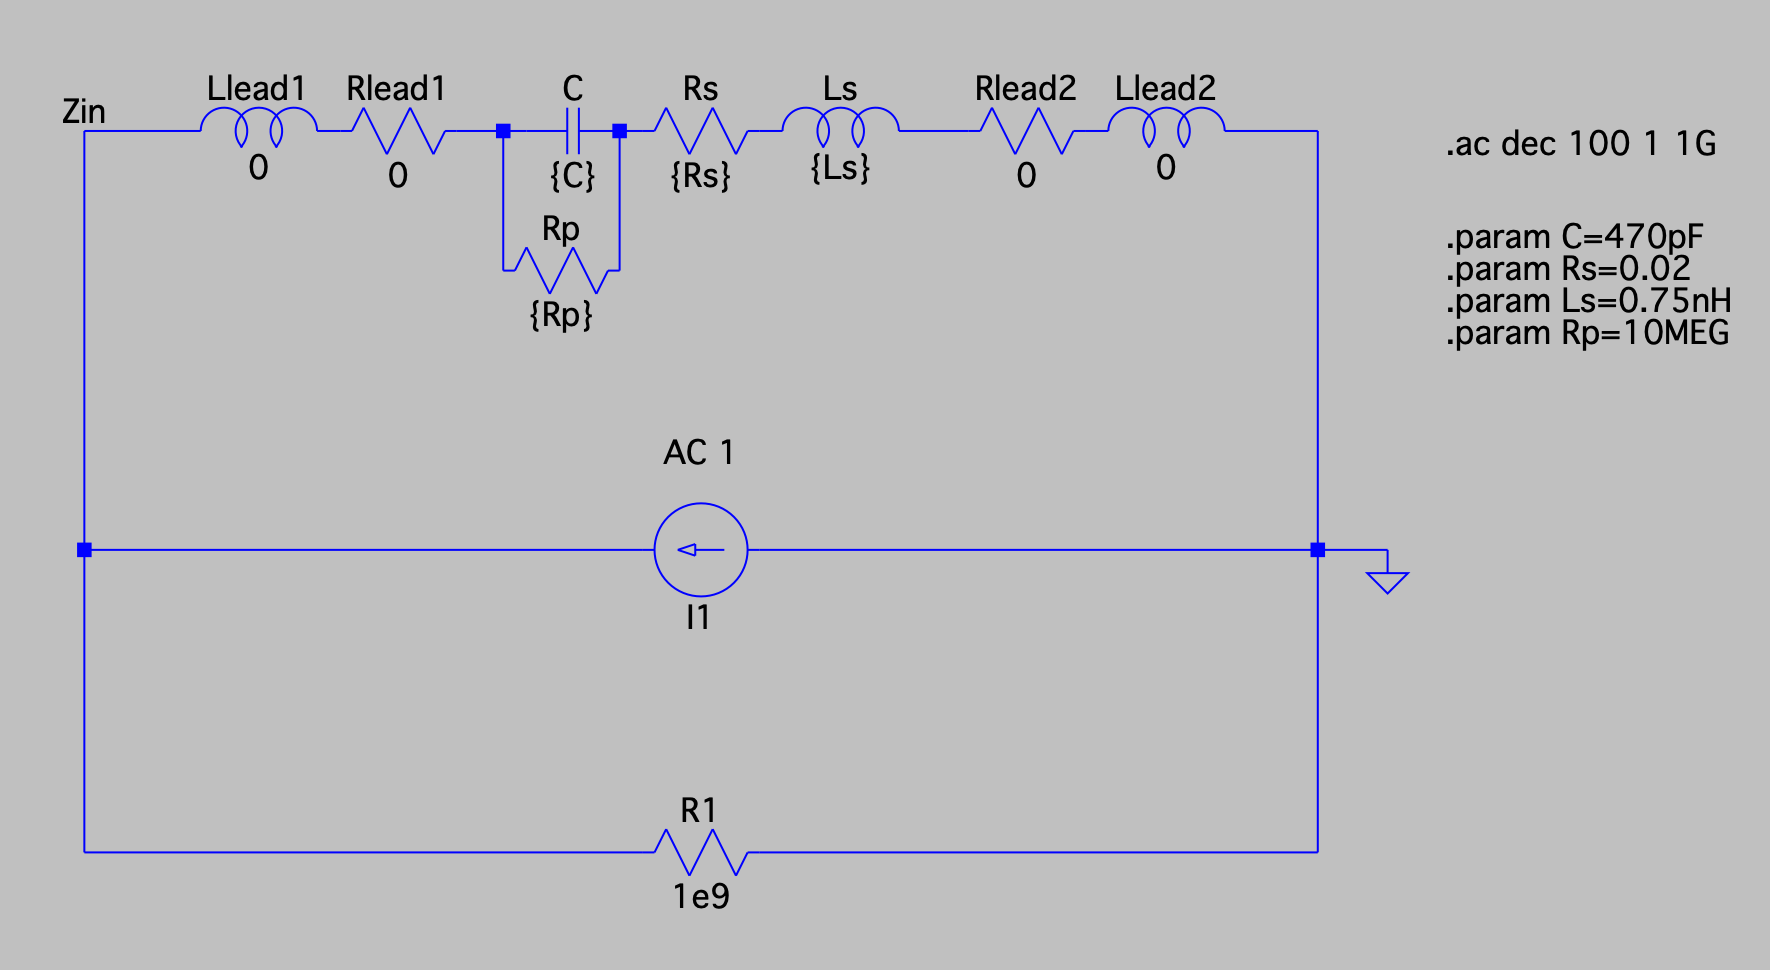
\includegraphics[width=12cm]{assets/cap_schematic.png}
\caption{Schematic of a non-ideal capacitor in LTSpice}
\end{figure}
\begin{figure}[h]
\centering
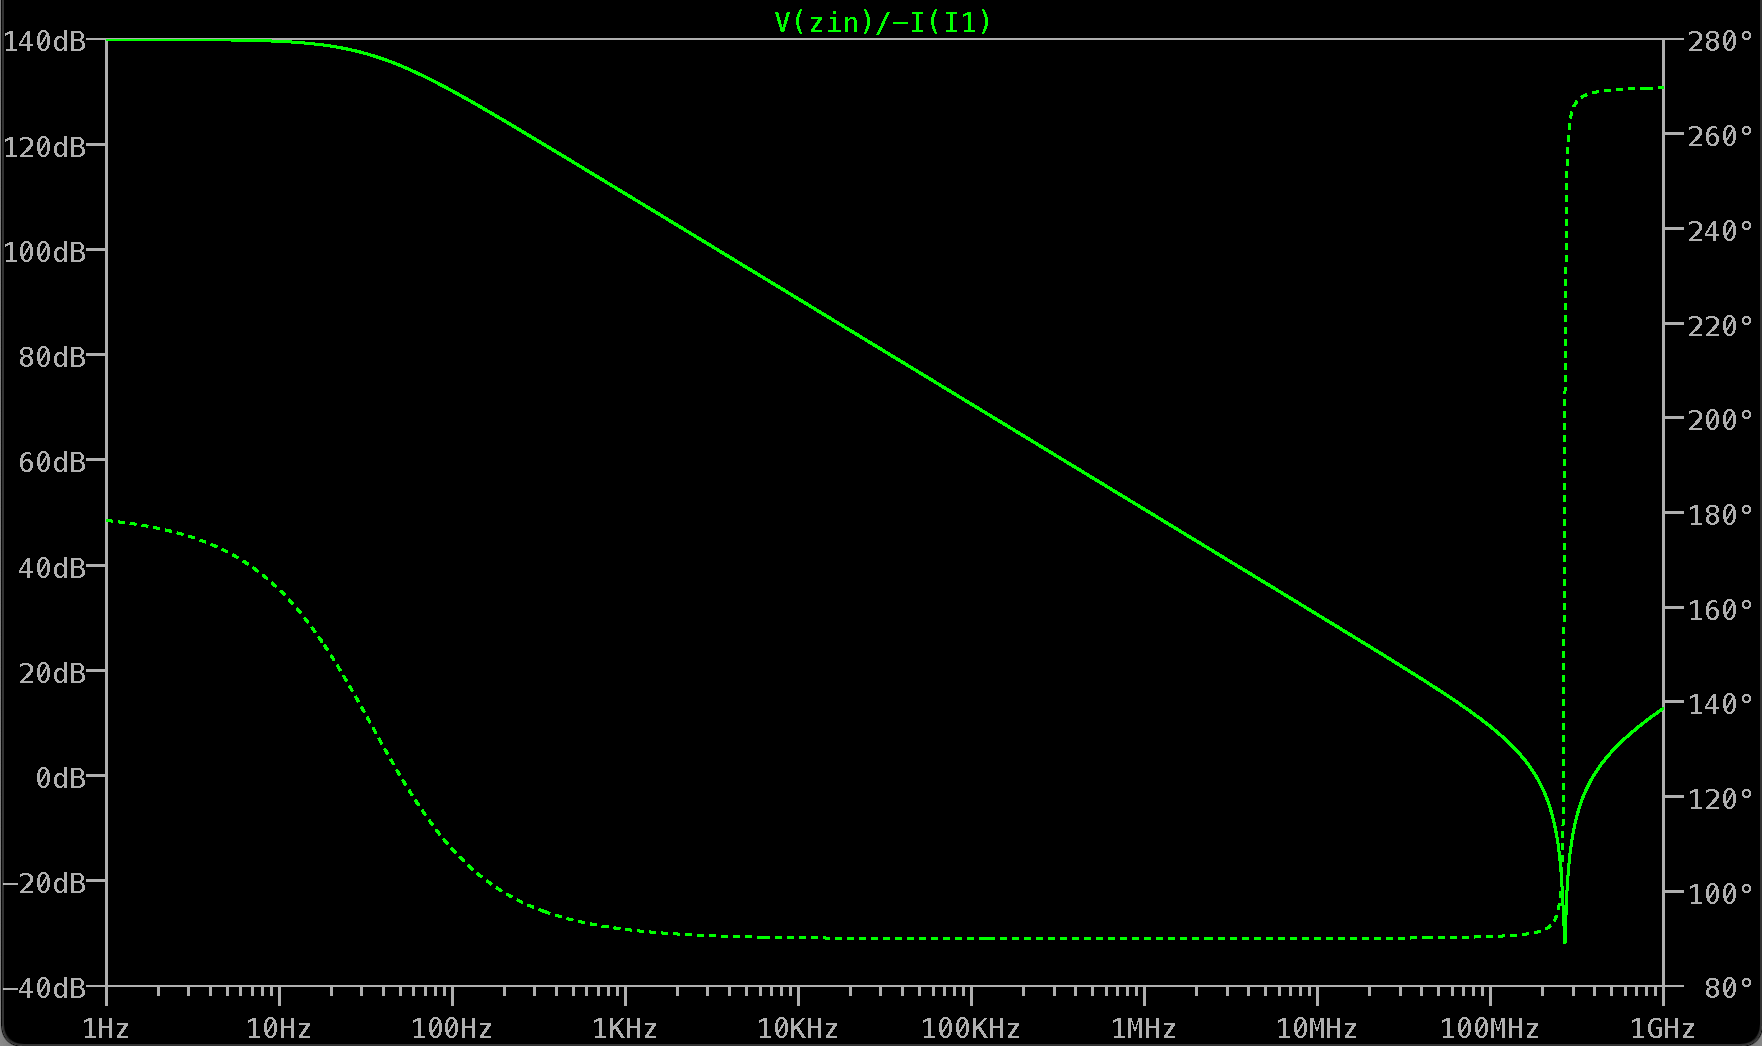
\includegraphics[width=12cm]{assets/cap_impedance.png}
\caption{Plot of impedance for capacitor in LTSpice}
\end{figure}
The plot shows that impedance start decreasing around 100Hz with a sharp dip around 250MHz. This dip is called the knee point and can be used to find the ESL in our capacitor. 
\begin{equation} 
     f = \frac{1}{2\cdot\pi\sqrt{\text{ESL}\cdot C}}
\end{equation}

\subsection*{Inductor}
The inductor I used in lab was a 2929SQ-331 inductor which has a value of 330 nH.  
\begin{figure}[h]
\centering
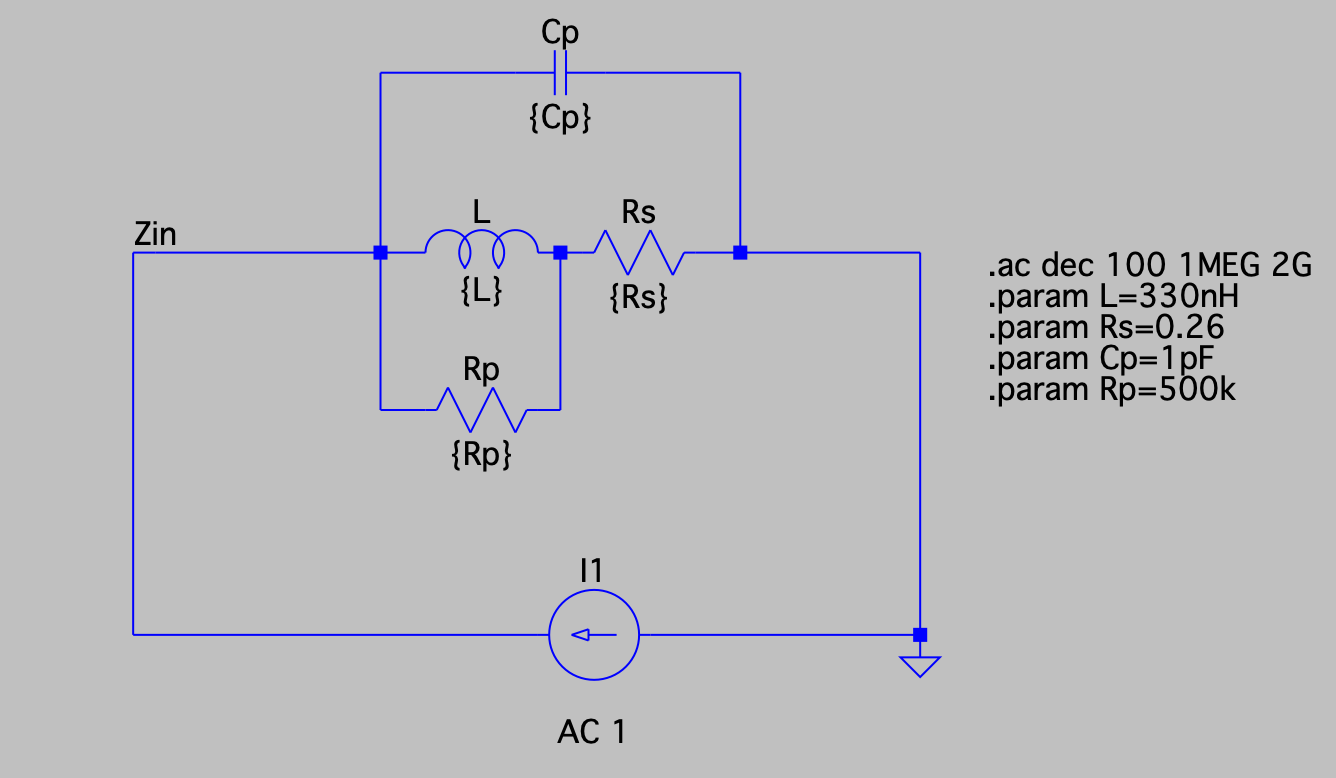
\includegraphics[width=12cm]{assets/ind_schematic.png}
\caption{Schematic of a non-ideal inductor in LTSpice}
\end{figure}
\begin{figure}[h]
\centering
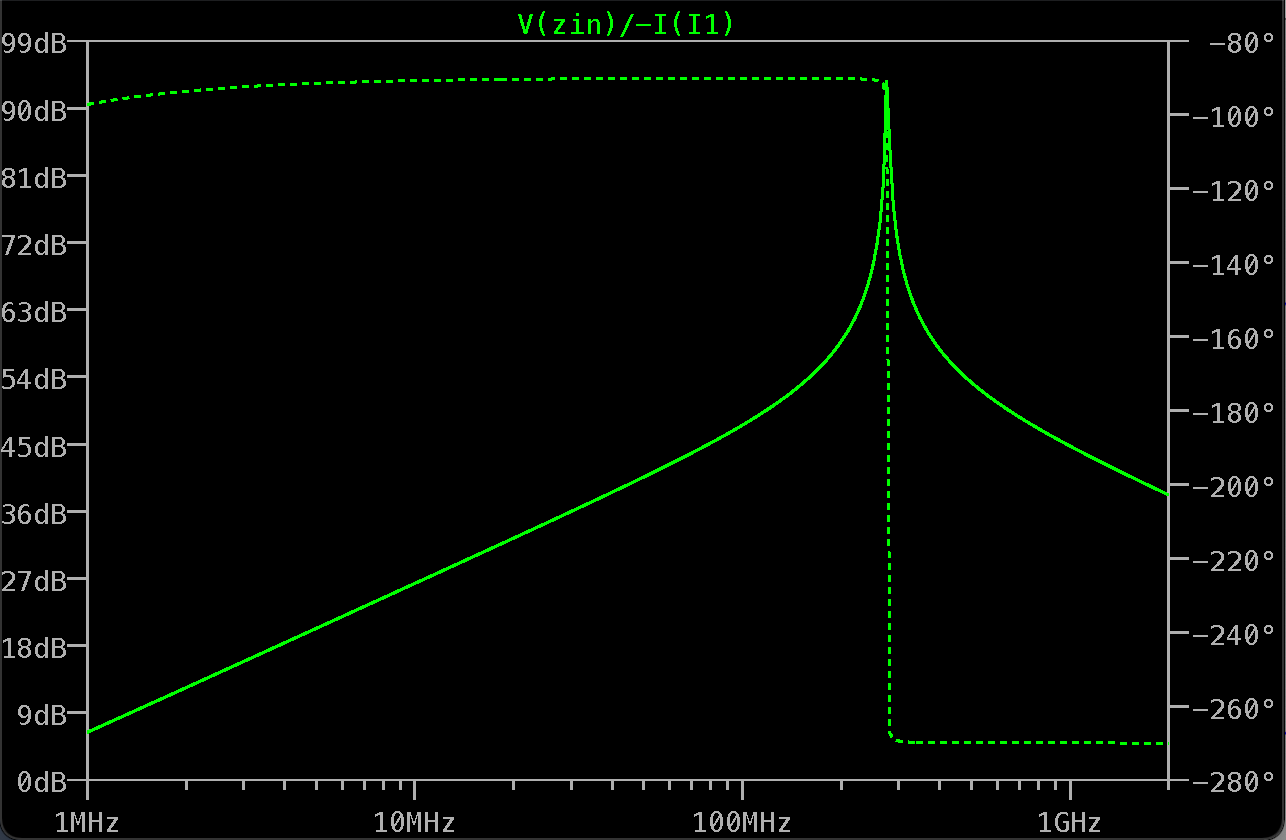
\includegraphics[width=12cm]{assets/ind_impedance.png}
\caption{Plot of impedance for inductor in LTSpice}
\end{figure}
The plot in this case shows a sharp peak in impedance around 275MHz aka the self-resonance frequency. The equivalent parallel capacitance can be found using equation [2] which is the same as the one we used for the ESL in the capacitor. 
\begin{equation}
     f = \frac{1}{2\cdot\pi\sqrt{\text{EPC}\cdot L}}
\end{equation}
Below 275MHz, the inductor acts normally with impedance increasing with increasing frequency. Over 275MHz, the inductor acts like a capacitor with impedance decreasing with increasing frequency. We will see this come into play when we use a VNA and look at the resulting Smith Chart from our inductor. 
\clearpage
\section*{Lab Measurements}
\subsection*{Capacitor}
Below is the VNA measurement of a 470pF capacitor, you can see on the Smith chart that the line crosses the horizontal axis twice indicating that there are two resonant frequencies. The chart also indicates that at certain frequencies, the capacitor will act as an inductor like we found in our LTSpice simulations. 
\begin{figure}[h!]
\centering
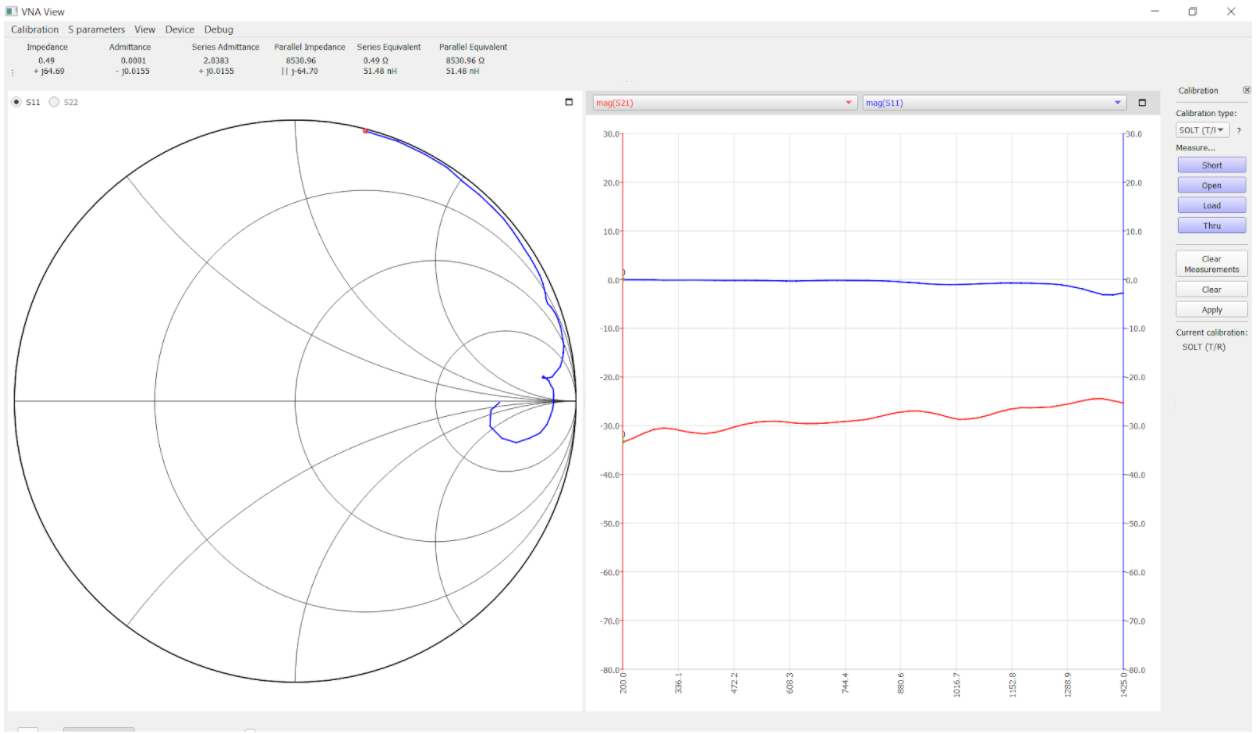
\includegraphics[width=12cm]{assets/cap_measurement.png}
\caption{VNA measurement of capacitor}
\end{figure}
\subsection*{Inductor}
The next item we measured with the VNA was a 330nH inductor. Here we see that the inductor again has multiple self-resonance frequencies and can act either as a capacitor or inductor.  
\begin{figure}[h]
\centering
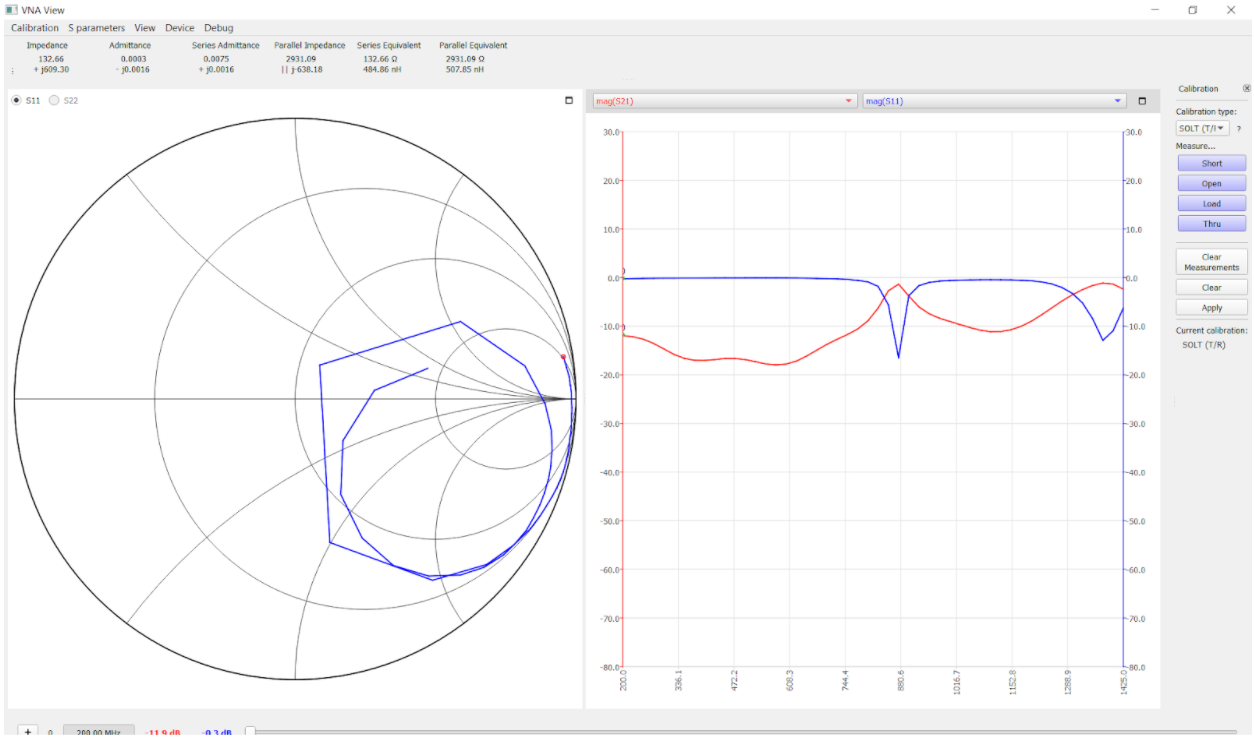
\includegraphics[width=12cm]{assets/ind_measurement.png}
\caption{VNA measurement of inductor}
\end{figure}

\end{document}
